\documentclass[12pt,a4paper]{article}
\usepackage{ucebnice}

\title{Základní matematické poznatky}
\author{Ondřej Škubala}
\date{\today}

\begin{document}

\maketitle
\newpage

\section{Množiny}
\begin{quotebox}
{„Množina je souhrn objektů, které jsou přesně určené a rozlišitelné
 a tvoří součást světa našich představ a myšlenek; tyto objekty nazýváme prvky množiny.“}
{Georg Cantor}
\end{quotebox}

\begin{historicalbox}
Množinové představy intuitivně užívali již staří řečtí matematici
ve 3. stol. př. n. l., například při zkoumání
\important{geometrických míst bodů} – tedy množin všech 
bodů daných vlastností (například kružnice jako množina 
všech bodů se stejnou vzdáleností od středu).  

\smallskip
K vytvoření samotné teorie množin přispěl i často zapomínaný český matematik, 
filosof a teolog \textbf{Bernard Bolzano} (1781–1848) 
svým dílem \emph{Paradoxy nekonečna}. Pojem \emph{teorie množin} 
však zavedl až německý matematik \textbf{Georg Cantor} (1845–1918), 
který od roku 1870 systematicky studoval problémy 
týkající se nekonečných množin reálných čísel.  

\smallskip
\textbf{Bernard Bolzano (1781–1848)} ve svém díle \emph{Paradoxy nekonečna} 
předběhl dobu, když se zabýval otázkami nekonečna.  

\smallskip
\textbf{Georg Cantor (1845–1918)} je považován za zakladatele teorie množin. 
Jako první zkoumal různé druhy nekonečna a ukázal, že existuje např. 
rozdíl mezi množinou všech přirozených čísel a množinou všech reálných čísel.

\smallskip
Symbol $\in$ pro „patří do“ zavedl \textbf{Giuseppe Peano} (1858–1932). 
Značku pro prázdnou množinu $\emptyset$ používáme až od 20. století, 
kdy ji zavedla skupina matematiků známá jako \textbf{Bourbaki}.
\end{historicalbox}


Množina, jak je z citátu G. Cantora zřejmé, je tedy \textbf{souhrn objektů}, 
u kterých lze vždy rozhodnout, zda do daného souhrnu patří či nikoli. 
Množiny značíme obvykle velkými písmeny, např. $A$, $B$, $M$, 
a jejich prvky naopak malými písmeny, např. $a$, $b$, $m$.

Se základními množinami jste se setkali už na základní škole – například s množinou všech přirozených čísel.  
Pojem \important{množina} není možné jednoduše a 
naprosto přesně definovat, protože tvoří jeden z 
\emph{prvotních pojmů matematiky}. Proto se spokojíme s intuitivním vysvětlením:  

\begin{definitionbox}
\important{Množina} je souhrn nějakých předmětů (objektů), které dohromady tvoří tuto množinu.  
Jednotlivé předměty množiny nazýváme \important{prvky množiny}.
\end{definitionbox}

\begin{examplebox}
\begin{itemize}
    \item $A = \{1,2,3,4,5\}$ je množina přirozených čísel od 1 do 5.  
    \item $B = \{x \in \mathbb{N} \mid x \text{ je sudé a } x < 10\} = \{2,4,6,8\}$.
\end{itemize}
\end{examplebox}


Jednou z oficiálních definic množin je například tato:
\begin{definitionbox}
\textbf{Definice}: \emph{Základní operace na množinách}

Nechť $a, b$ jsou množiny. Pak platí:
\begin{enumerate}
    \item $a \cup b = \{x : x \in a \lor x \in b\}$ \quad (sjednocení dvou množin),
    \item $a \cap b = \{x : x \in a \land x \in b\}$ \quad (průnik dvou množin),
    \item $\mathcal{P}(a) = \{x : x \subseteq a\}$ \quad (mocninná množina – množina všech podmnožin $a$),
    \item $S_a = \{x : (\exists t)(t \in a \land x \in t)\}$ \quad (suma – sjednocení všech prvků $a$),
    \item $a \times b = \{(x,y) : x \in a \land y \in b\}$ \quad (kartézský součin),
    \item $a^b = \{ f \mid f : b \to a \text{ je funkce} \}$ \quad (množina všech funkcí z $b$ do $a$).
\end{enumerate}
\end{definitionbox}
Jak je možné si všimnout, není zcela triviální. Tudíž pro naši potřebu bohatě postačuje 
představa množiny jako pytlíčku různých věcí.

\subsubsection*{Způsoby zápisu množin}

Množinu můžeme zapsat a určit buď pomocí \important{výčtu prvků}, nebo pomocí \important{charakteristiky}.  
U výčtu prvků zapisujeme množinu do složených závorek a vypisujeme \textbf{všechny} prvky, které množina obsahuje.  
Když zapisujeme množinu charakteristikou, využíváme \important{výrokové formy} k vyjádření dané množiny.

\begin{itemize}
    \item \textbf{Výčtem prvků:} všechny prvky množiny vypíšeme do složených závorek.
    \[
    A = \{1,2,3,4,5\}
    \]

    \item \textbf{Charakteristikou (předpisem):} uvedeme vlastnost, kterou prvky množiny splňují.
    \[
    B = \{x \in \mathbb{N} \mid x < 6\}
    \]
\end{itemize}

\begin{examplebox}
    Zde je příklad jak zaspat tu stejnou množinu $C$ charakteristikou a poté výčtem prvků:
    \[
    C = \{x \in \mathbb{Z} \mid -2 \leq x \leq 2\}
    \]
    
    \[
    C = \{-2,-1,0,1,2\}
    \]

\end{examplebox}

\subsection{Druhy množin}

Množiny se mohou lišit podle toho, kolik obsahují prvků. 
Některé mají prvků jen pár a můžeme je snadno vypsat, 
jiné jich mají nekonečně mnoho a není možné je všechny vypsat. 
A existuje i zvláštní případ, kdy množina nemá žádný prvek.  

\begin{itemize}
    \item \textbf{Konečná množina} má jen konečný počet prvků.  
    Příkladem je $\{1,2,3\}$ – tuto množinu dokážeme vypsat celou.
    
    \item \textbf{Nekonečná množina} má nekonečně mnoho prvků.  
    Typickým příkladem je množina všech přirozených čísel $\mathbb{N} = \{1,2,3,4,\dots\}$.  
    Takovou množinu nikdy nevyčerpáme výčtem.

    \item \textbf{Prázdná množina} je množina bez jediného prvku.  
    Značíme ji
    \[
    \emptyset \quad \text{nebo} \quad \{\}.
    \]  
    Prázdnou množinu můžeme chápat jako „pytlík, ve kterém nic není“.
\end{itemize}

\begin{examplebox}
\begin{itemize}
    \item $\{x \in \mathbb{Z} \mid x^2 < 10\} = \{-3,-2,-1,0,1,2,3\}$ je \textbf{konečná množina}.  
    \item $\{x \in \mathbb{N} \mid x \text{ je sudé}\} = \{2,4,6,8,\dots\}$ je \textbf{nekonečná množina}.  
    \item $\{x \in \mathbb{Z} \mid x^2 = -1\} = \emptyset$ je \textbf{prázdná množina}.
\end{itemize}
\end{examplebox}

\subsubsection*{Rovnost množin}
Říkáme, že dvě množiny $A$ a $B$ jsou \emph{rovny}, jestliže obsahují \textbf{stejné prvky}.  
Nezáleží na pořadí, v jakém jsou prvky zapsány, ani na jejich opakování.  

\begin{examplebox}
Platí $\{1,2,3\} = \{3,2,1,2\}$, protože obě množiny obsahují právě prvky $1,2,3$.  
\end{examplebox}


\subsubsection*{Podmnožiny}
Říkáme, že množina $A$ je \emph{podmnožinou} množiny $B$, jestliže každý prvek $A$ je zároveň prvkem $B$.  
Značíme:
\[
A \subseteq B
\]

\begin{examplebox}
Množina $\{1,2,3\}$ je podmnožinou množiny $\{1,2,3,4,5\}$, tedy $\{1,2,3\} \subseteq \{1,2,3,4,5\}$.
\end{examplebox}

Pokud $A \subseteq B$ a zároveň $A \neq B$, říkáme, že $A$ je \emph{vlastní podmnožinou} množiny $B$.  
Naopak pokud $A = B$, pak $A$ je podmnožinou $B$, ale nikoli vlastní podmnožinou.

\begin{examplebox}
\begin{itemize}
    \item $\{1,2\} \subseteq \{1,2,3\}$ – vlastní podmnožina.  
    \item $\{1,2,3\} \subseteq \{1,2,3\}$ – podmnožina, ale \textbf{ne} vlastní.
\end{itemize}
\end{examplebox}


\subsubsection*{Ilustrace}

Množiny můžeme zapisovat tedy \textbf{textově}, anebo \textbf{graficky} pomocí množinových diagramů, tzv. \important{Vennových diagramů}.  
Tyto diagramy napomáhají nejen v názorném znázornění vztahů mezi množinami, ale také při řešení různých slovních úloh.  

\begin{center}
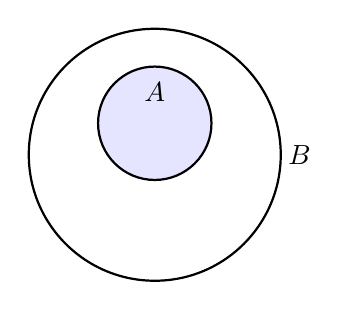
\begin{tikzpicture}[scale=0.8]
  % velká množina B
  \draw[thick] (0,0) circle (2);
  \node at (2.3,0) {$B$};
  % menší množina A
  \draw[thick, fill=blue!10] (0,0.5) circle (0.9);
  \node at (0,1) {$A$};
\end{tikzpicture}
\hspace{2.5cm}
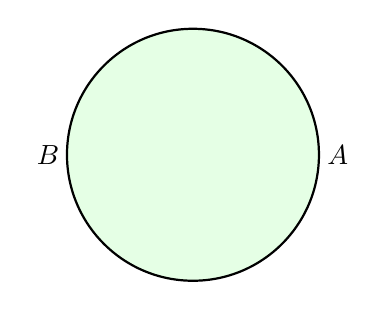
\begin{tikzpicture}[scale=0.8]
  % množina A = B
  \draw[thick, fill=green!10] (0,0) circle (2);
  \node at (2.3,0) {$A$};
  \node at (-2.3,0) {$B$};
\end{tikzpicture}
\end{center}

\begin{center}
Vlevo: $A \subseteq B$ (podmnožina).  
Vpravo: $A = B$ (rovnost množin).
\end{center}

\subsection{Mohutnost množiny}

Počet prvků v konečné množině nazýváme \important{mohutností množiny} (též kardinalitou).  
Značíme ji svislými čarami: $|A|$.  

\begin{definitionbox}
Nechť $A$ je konečná množina. Potom \textbf{mohutnost množiny $A$} je číslo udávající počet jejích prvků:  
\[
|A| = n \quad \Leftrightarrow \quad A \text{ má právě $n$ prvků}.
\]
\end{definitionbox}

\begin{examplebox}
\begin{itemize}
    \item $A = \{1,2,3,4,5\}$ má $|A| = 5$.  
    \item $B = \{\text{pondělí, úterý, středa}\}$ má $|B| = 3$.  
    \item $C = \emptyset$ má $|C| = 0$.
\end{itemize}
\end{examplebox}


\subsubsection*{Nekonečné množiny}

U konečných množin můžeme jejich prvky vypsat a spočítat, kolik jich je.  
Naproti tomu existují množiny, které prvků obsahují \emph{nekonečně mnoho}.  
Počet prvků těchto množin se nedá vyjádřit žádným konečným číslem – říkáme, že jejich mohutnost je \textbf{nekonečná}.  

\newpage
\begin{examplebox}
\begin{itemize}
    \item $\mathbb{N} = \{1,2,3,4,5,\dots\}$ – množina všech přirozených čísel.  
      Nemá poslední prvek a vždy k ní můžeme přidat ještě další číslo.  
    \item $\mathbb{Z} = \{\dots,-3,-2,-1,0,1,2,3,\dots\}$ – množina všech celých čísel.  
    \item $\mathbb{Q}$ – množina všech racionálních čísel (zlomků) je také nekonečná, i když mezi každými dvěma čísly existuje nekonečně mnoho dalších zlomků.  
\end{itemize}
\end{examplebox}

\paragraph{Poznámka.} Nekonečno není „velmi velké číslo“. Je to odlišný pojem – žádné konečné číslo, byť obrovské, se mu nevyrovná.  
Například pokud z $\mathbb{N}$ odebereme jen několik málo čísel (třeba $1,2,3$), zůstane nám stále nekonečná množina.  

\begin{notebox}
\textbf{Zajímavost:} Německý matematik Georg Cantor (1845–1918) objevil, že existují \emph{různě velká nekonečna}.  
Například:
\begin{itemize}
    \item množina všech přirozených čísel $\mathbb{N} = \{1,2,3,\dots\}$ je nekonečná, ale \emph{spočitatelná},  
    \item množina všech reálných čísel $\mathbb{R}$ je nekonečná a navíc \emph{nespočitatelná}.  
\end{itemize}
Cantor dokázal, že mezi $\mathbb{N}$ a $\mathbb{R}$ není možné vytvořit vzájemně jednoznačné přiřazení (tzv. bijekci).  
Proto říkáme, že $|\mathbb{R}|$ je \textbf{větší nekonečno} než $|\mathbb{N}|$.
\end{notebox}



\subsection{Množinové operace}
\subsubsection*{Doplněk množiny}

V případě, že množina $B$ je podmnožinou množiny $A$, zavádíme pojem \important{doplněk množiny $B$ v množině $A$}.  
Zapisujeme jej jako $B'_A$ a rozumíme tím množinu všech prvků z $A$, které nepatří do $B$:  

\begin{definitionbox}
\[
B'_A = \{x \in A \mid x \notin B\}.
\]
\end{definitionbox}

\begin{examplebox}
Nechť $A = \{1,2,3,4,5,6,7,8,9,10\}$ a $B = \{2,4,6,8,10\}$.  
Pak doplněk množiny $B$ v $A$ je
\[
B'_A = \{1,3,5,7,9\}.
\]
\end{examplebox}

\subsubsection*{Průnik množin}

Často nás zajímá, které prvky mají dvě množiny společné.  
Tuto množinu nazýváme \important{průnikem množin} a značíme $A \cap B$.  

\begin{definitionbox}
\textbf{Průnik množin} $A$ a $B$ je množina všech prvků, které patří zároveň do $A$ i do $B$:  
\[
A \cap B = \{x \mid x \in A \land x \in B\}.
\]
\end{definitionbox}

\begin{examplebox}
Nechť $A = \{1,2,3,4,5\}$ a $B = \{3,4,5,6,7\}$.  
Pak
\[
A \cap B = \{3,4,5\}.
\]
\end{examplebox}


\subsubsection*{Sjednocení množin}

Někdy nás zajímá celá množina všech prvků, které leží alespoň v jedné z množin.  
Tuto množinu nazýváme \important{sjednocením množin} a značíme $A \cup B$.  

\begin{definitionbox}
\textbf{Sjednocení množin} $A$ a $B$ je množina všech prvků, které patří do $A$ nebo do $B$ (případně do obou):  
\[
A \cup B = \{x \mid x \in A \lor x \in B\}.
\]
\end{definitionbox}

\begin{examplebox}
Nechť $A = \{1,2,3,4,5\}$ a $B = \{3,4,5,6,7\}$.  
Pak
\[
A \cup B = \{1,2,3,4,5,6,7\}.
\]
\end{examplebox}


\subsubsection*{Rozdíl množin}

Další často používanou operací je \important{rozdíl množin}.  
Rozdílem množin $A$ a $B$ rozumíme všechny prvky, které jsou v $A$, ale \textbf{nejsou} v $B$.  
Rozdíl značíme $A \setminus B$.  

\begin{definitionbox}
\textbf{Rozdíl množin} $A$ a $B$ je množina všech prvků, které patří do $A$, ale nepatří do $B$:  
\[
A \setminus B = \{x \mid x \in A \land x \notin B\}.
\]
\end{definitionbox}

\begin{examplebox}
Nechť $A = \{1,2,3,4,5\}$ a $B = \{3,4,5,6,7\}$.  
Pak
\[
A \setminus B = \{1,2\}, \quad B \setminus A = \{6,7\}.
\]
\end{examplebox}

\newpage
\subsection{Množinové operace – shrnutí}

\begin{center}
\renewcommand{\arraystretch}{1.6}
\setlength{\tabcolsep}{10pt}
\begin{tabular}{|p{2,5cm}|p{1,5cm}|p{5cm}|c|}
\hline
\rowcolor{pastelblue!60}
\textbf{Název} & \textbf{Značení} & \textbf{Definice} & \textbf{Vennův diagram} \\
\hline


\important{Průnik}    
 & $A \cap B$ &
Množina všech prvků, které patří současně do $A$ i $B$. &
\begin{tikzpicture} 
% Set A
\node [draw, circle, minimum size =2cm, label={135:$A$}] (A) at (0,0){}; ;
 
% Set B
\node [draw, circle, minimum size =2cm, label={45:$B$}] (B) at (1.2,0){};
 
% Intersection
\begin{scope}
    \clip (0,0) circle(1cm);
    \clip (1.2,0) circle(1cm);
    \fill[pastelblue](0,0) circle(1cm);
\end{scope}
 
% Circles outline
\draw (0,0) circle(1cm);
\draw (1.2,0) circle(1cm);
 
% Set intersection label
% \node at (0.6,-1.2) {$A\cap B$};
\end{tikzpicture} \\
\hline


\important{Sjednocení} & $A \cup B$ &
Množina všech prvků, které patří alespoň do jedné z množin $A$, $B$. &
\begin{tikzpicture} 
    % Set A 
    \node [circle, fill=pastelorange, minimum size =2cm, label={135:$A$}] (A) at (0,0){}; 
    % Set B 
    \node [circle, fill=pastelorange, minimum size =2cm, label={45:$B$}] (B) at (1.2,0){}; 
    % Circles outline 
    \draw[black,thick] (0,0) circle(1cm); 
    \draw[black,thick] (1.2,0) circle(1cm); 
    % Union text label 
    % \node[orange!90!black] at (0.9,1.8) {$A\cup B$}; 
\end{tikzpicture} \\
\hline

\important{Rozdíl} & $A \setminus B$ &
Množina všech prvků, které patří do $A$, ale nepatří do $B$. &
\begin{tikzpicture}[thick, set/.style = { circle, minimum size = 2cm}] 
    % Set A 
    \node[set,fill=pastelgreen,label={135:$A$}] (A) at (0,0) {}; 
    % Set B 
    \node[set,fill=white,label={45:$B$}] (B) at (0:1.2) {}; 
    % Circles outline 
    \draw (0,0) circle(1cm); 
    \draw (1.2,0) circle(1cm); 
    % Difference text label 
    %\node[left,black] at (0.35,0){$A-B$}; 
\end{tikzpicture} \\
\hline

\important{Doplněk} & $A'$ &
Množina všech prvků základní množiny $U$, které nepatří do $A$. &
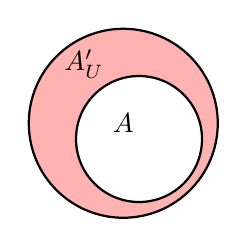
\begin{tikzpicture}[thick]
  % univerzum jako větší kruh
  \fill[red!30] (0,0) circle (1.2);
  \draw (0,0) circle (1.2);
  % množina A uvnitř
  \fill[white] (0.2,-0.2) circle (0.8cm);
  \draw (0.2,-0.2) circle (0.8cm);
  \node at (0,0) {$A$};
  \node at (-0.5,0.75) {$A'_U$};
  % popisek doplňku
  % \node[red!80!black] at (0,-1.7) {$A'$};
\end{tikzpicture} \\
\hline


\end{tabular}
\end{center}


\newpage
\subsection{Vennovy diagramy}

\begin{notebox}
\textbf{Vennův diagram} je grafické znázornění vztahů mezi množinami.  
Jednotlivé množiny znázorňujeme kruhy.  
Jejich průniky (překryvy) znázorňují prvky, které patří do více množin současně.  
Pomocí Vennových diagramů lze názorně řešit i složitější slovní úlohy.
\end{notebox}

\subsubsection*{Dvě množiny}
Pokud máme dvě množiny $A$ a $B$, Vennův diagram tvoří dva překrývající se kruhy:

\begin{center}
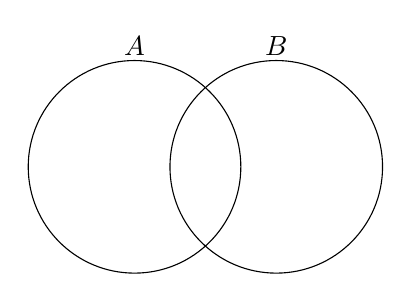
\begin{tikzpicture}[scale=0.9]
  \draw (-1,0) circle (1.5);
  \draw ( 1,0) circle (1.5);
  \node at (-1,1.7) {$A$};
  \node at ( 1,1.7) {$B$};
\end{tikzpicture}
\end{center}

\subsubsection*{Tři množiny}
Při třech množinách $A, B, C$ už máme tři kruhy uspořádané do tvaru trojlístku:

\begin{center}
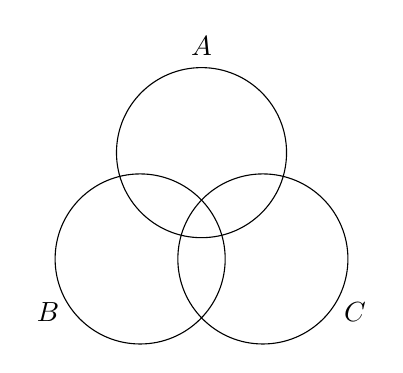
\begin{tikzpicture}[scale=0.9]
  \draw (90:1) circle (1.2);
  \draw (210:1) circle (1.2);
  \draw (330:1) circle (1.2);
  \node at (90:2.5) {$A$};
  \node at (210:2.5) {$B$};
  \node at (330:2.5) {$C$};
\end{tikzpicture}
\end{center}

\subsubsection*{Příklad – práce s Vennovým diagramem}
\begin{examplebox}
Nechť \[U = \{1,2,3,4,5,6,7,8,9\}\] je základní množina všech přirozených čísel menších než 10.  

Definujme:  
\[
A = \{x \in U \mid 3 \text{ dělí } x\}, \qquad
B = \{x \in U \mid x \text{ je sudé}\}.
\]

Pak:
\[
A = \{3,6,9\}, \qquad
B = \{2,4,6,8\}.
\]


Zapiš množiny $A \cap B$, $A \cup B$, $A \setminus B$, $B \setminus A$ a $\overline{A}$.
\end{examplebox}

\begin{solutionbox}
\begin{align*}
A \cap B &= \{6\}, \\
A \cup B &= \{2,3,4,6,8,9\}, \\
A \setminus B &= \{3,9\}, \\
B \setminus A &= \{2,4,8\}, \\
\overline{A} &= U \setminus A = \{1,2,4,5,7,8\}.
\end{align*}


\begin{center}
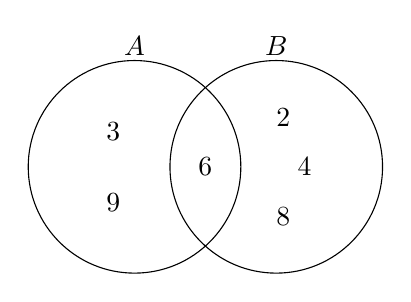
\begin{tikzpicture}[scale=0.9]
  % Množina A
  \draw (-1,0) circle (1.5);
  \node at (-1,1.7) {$A$};
  % Množina B
  \draw ( 1,0) circle (1.5);
  \node at ( 1,1.7) {$B$};
  
  % popisky prvků
  \node at (-1.3,0.5) {3};
  \node at (-1.3,-0.5) {9};
  \node at ( 1.1,0.7) {2};
  \node at ( 1.4,-00) {4};
  \node at ( 1.1,-0.7) {8};
  \node at ( 0,0) {6}; % průnik
\end{tikzpicture}
\end{center}
\end{solutionbox}


% -----------------------------------------------------------------
% ---------------------- P Ř Í K L A D Y --------------------------
% -----------------------------------------------------------------


\exercisepart


\begin{exercise}
Zapište všechny podmnožiny množin:
\begin{tasks}(2)
    \task $\{2;7\}$
    \task $\{5;7;9\}$
    \task $\emptyset$
    \task $\{0\}$
    \task $\{1;2;3;5\}$
    \task $\{\{1;2\}; 3 \}$
\end{tasks}
\end{exercise}


\begin{exercise}
Nechť $A = \{-3,0,0{,}5,1\}$.  
Zapište všechny podmnožiny množiny $A$, které jsou zároveň podmnožinami následujících množin:
\begin{enumerate}[label=\alph*)]
    \item množiny přirozených čísel $\mathbb{N}$,
    \item množiny celých čísel $\mathbb{Z}$,
    \item množiny $\{x \in \mathbb{R} \mid |x| < 1\}$.
\end{enumerate}
\end{exercise}


% 2. úkoly
\setcounter{section}{2}
\begin{exercise}
Určete doplněk množiny $B$ v množině $A$, tj.
\[
B'_A = \{x \in A \mid x \notin B\},
\]
pro následující dvojice množin:
\begin{enumerate}[label=\alph*)]
    \item $A = \{-2,-0.5,0,1,3\}, \quad B = \{-0.5,0,3\}$
    \item $A = \mathbb{Z}, \quad B = \{x \in \mathbb{Z} \mid x \leq 0\}$
    \item $A = \{x \in \mathbb{Z} \mid x > 5\}, \quad B = \{x \in \mathbb{Z} \mid x \geq 7\}$
    \item $A = \mathbb{N}, \quad B = \{x \in \mathbb{N} \mid x \text{ je sudé}\}$
    \item $A = \mathbb{Z}, \quad B = \{x \in \mathbb{Z} \mid |x| \geq 2\}$
    \item $A = \mathbb{R}, \quad B = \{x \in \mathbb{R} \mid x^2 \leq -x\}$
    \item $A = \mathbb{R}, \quad B = \{x \in \mathbb{R} \mid |x-2| \geq 0\}$
    \item $A = \mathbb{R}, \quad B = \{x \in \mathbb{R} \mid |x| < 0\}$
\end{enumerate}
\end{exercise}


\begin{exercise}
Mějme množiny $A=\langle -7,2\rangle $, $B=\langle-2,5)$, $C=\langle2,\infty)$ v $\mathbb{R}$. Zapište:
\begin{tasks}(4)
    \task $A \cap B$
    \task $A \cap C$
    \task $A \cup B$
    \task $(A \cap B) \cup C$
    \task $(A \cup B) \cup C$
    \task \smash{$(A \cap C) \cup (B \cap C) $}
    \task $A'_{\mathbb{R}}$
    \task $A \setminus B$
\end{tasks}
\end{exercise}


\begin{exercise}
Určete, které z následujících množin jsou si rovny:
\begin{tasks}(2)
    \task $\{ \text{všechna přirozená čísla menší než $0$}\}$,
    \task $\{0\}$,
    \task $\{x \in \mathbb{R} \mid -2 \leq x \leq 2\}$,
    \task $\{-2,-1,0,1,2\}$,
    \task $\emptyset$,
    \task $\{x \in \mathbb{Z} \mid -3 < x < 3\}$,
    \task $\{x \in \mathbb{R} \mid |x| \leq 0\}$,
    \task $\{x \in \mathbb{R} \mid  x^2 + 1 = 0\} $
\end{tasks}
\end{exercise}


\begin{exercise}
Stanovte podmínky, které musí být splněny, aby platilo:
\begin{enumerate}[label=\alph*)]
    \item $A \cap B = A$
    \item $A \cup B = A$
    \item $B'_A = A$
    \item $B'_A=\emptyset$
    \item $A \cup B = A \cap B$
\end{enumerate}
\end{exercise}


\begin{exercise}
Mějme univerzum $U = \mathbb{Z}$, tedy množinu všech celých čísel.  
Určete doplňky následujících množin v $U$:
\begin{enumerate}[label=\alph*)]
    \item $A = \{x \in \mathbb{Z} \mid x < 1\}$,
    \item $B = \mathbb{N}$,
    \item $C = \{x \in \mathbb{Z} \mid \sqrt{x^2} = |x|\}$,
    \item $D = \{x \in \mathbb{Z} \mid |x| > 0\}$.
\end{enumerate}
\end{exercise}


\begin{exercise}
Určete průniky následujících množin $A$ a $B$:
\begin{enumerate}[label=\alph*)]
    \item $A = \{1,2,3,4,5\}, \quad B = \{3,4,5,6,7\}$,
    \item $A = \{x \in \mathbb{Z} \mid -5 \leq x \leq 5\}, \quad B = \{x \in \mathbb{Z} \mid x \text{ je sudé}\}$,
    \item $A = \{a,e,i,o,u\}, \quad B = \{a,b,c,d,e\}$,
    \item $A = \mathbb{N}, \quad B = \{1,3,5,7,\dots\}$,
    \item $A = \{x \in \mathbb{Z} \mid x^2 < 10\}, \quad B = \{-5,-4,\dots,5\}$.
\end{enumerate}
\end{exercise}


\begin{exercise}
Určete sjednocení množin $A$ a $B$ z předchozího příkladu.
\end{exercise}


\begin{exercise}
Určete rozdíly množin $A \setminus B$ a $B \setminus A$ z příkladu 4.
\end{exercise}


% 3. úkoly
\setcounter{section}{3}
\newpage
\begin{exercise}
Na číselné ose vyznačte a jako interval zapište tyto množiny:  

\begin{enumerate}[label=\alph*)]
    \item všechna reálná čísla mezi $-2$ a $3$ včetně obou koncových bodů,  
    \item všechna reálná čísla větší než $-7$ a menší nebo rovna $-1$,  
    \item všechna reálná čísla větší nebo rovna $5$ a menší než $9$,  
    \item všechna reálná čísla menší nebo rovna $-2$.  
\end{enumerate}
\end{exercise}


% 4. úkoly
\setcounter{section}{4}
\begin{exercise}
Pomocí Vennova diagramu ověřte (nebo vyvraťte), zda platí:
\[
A \cap (B \cap C) \;=\; (A \cap B) \cup (A \cap C).
\]
\end{exercise}


\begin{exercise}
Do Vennových diagramů vyznačte následující množiny (každou do samostatného obrázku):
\begin{enumerate}[label=\alph*)]
    \item $A \cap (B \cap C)$
    \item $(A \cap B) \cup C$
    \item $(A \cup B) \cap C$
    \item $(A \cap B) \setminus C$
    \item $(A \cup C) \setminus B$
    \item $(A \triangle B) \cap C$ \quad (symetrický rozdíl $A$ a $B$)
\end{enumerate}
\end{exercise}


% 5. úkoly
\setcounter{section}{5}
\begin{exercise}
Z 30 dotázaných studentů hovoří anglicky nebo německy 28 studentů.
Dvacet studentů ovládá nejvýše jeden z těchto jazyků.
Anglicky mluví o 6 studentů více než německy.
Určete:
\begin{enumerate}[label=\alph*)]
    \item kolik studentů mluví jen anglicky,
    \item kolik studentů mluví anglicky i německy.
\end{enumerate}
\end{exercise}


\begin{exercise}
K obědu byla svíčková s knedlíkem. Kuchařky u okénka se špinavým nádobím 
provedly výzkum vrácených talířů od hlavního jídla. Alespoň kus knedlíku vrátilo 
301 strávníků, kus knedlíku nebo maso dokonce 328 z nich. Ani kousek masa nebyl 
na 554 talířích, pouze maso nebo pouze knedlík vrátilo 250 obědvajících. Určete:
\begin{enumerate}[label=\alph*)]
    \item kolik lidí snědlo všechno,
    \item kolik strávníků tento den obědvalo,
    \item kolik obědvajících vrátilo maso i knedlíky.
\end{enumerate}
\end{exercise}


\begin{exercise}
Z 15 kontrolovaných lavic je poškrábaných nebo popsaných 14.
Deset lavic má nejvýše jeden druh poškození.
Poškrábaných lavic je o 3 více než popsaných.
Určete:
\begin{enumerate}[label=\alph*)]
    \item kolik lavic je jen poškrábaných,
    \item kolik lavic je poškrábaných i popsaných.
\end{enumerate}
\end{exercise}


\begin{exercise}
Známá rocková skupina vystoupila dvakrát. Ze 450 studentů se koncertu aspoň jednou zúčastnilo 290, právě jednou 200.
Počet studentů, kteří byli pouze na prvním koncertu, je třikrát větší než počet studentů, kteří byli pouze na druhém.
Určete:
\begin{enumerate}[label=\alph*)]
    \item kolik studentů bylo na prvním koncertu,
    \item kolik studentů bylo na druhém koncertu.
\end{enumerate}
\end{exercise}


\begin{exercise}
Při jednání současné Poslanecké sněmovny Parlamentu ČR byl proveden průzkum 
pracovního vytížení přítomných poslanců. Bylo zjištěno, že kromě sledování 
průběhu projednávání zákonů poslanci zvládají číst noviny, telefonovat a hrát hry 
na notebooku. Noviny čte 34 poslanců, telefonuje jich 36 a hrami na notebooku se 
baví 38 zastupitelů. Žádnou z těchto tří činností nevykonává a jednání sleduje 
35 poslanců. Pouze dva poslanci pak stíhají všechny tři činnosti najednou.  
Noviny a zároveň telefonování zvládá 6 poslanců a 3 poslanci zároveň čtou a hrají hry.  
Telefonuje nebo hraje hry 65 poslanců. Určete, kolik poslanců:  
\begin{enumerate}[label=\alph*)]
    \item pouze telefonuje,
    \item hraje hry nebo čte,
    \item dokáže vykonávat alespoň dvě z uvedených činností,
    \item je přítomno jednání sněmovny.
\end{enumerate}
\end{exercise}


\begin{exercise}
Písemná práce z matematiky, které se zúčastnilo 35 studentů, obsahovala tři úlohy.
Dva studenti vyřešili jen první úlohu a tři studenti jen druhou úlohu.
První a druhou úlohu vyřešilo 16 studentů, druhou a třetí 14 studentů.
Všechny tři úlohy vyřešilo 10 studentů, první nebo třetí 31 studentů
a 3 studenti nevyřešili ani první, ani druhou úlohu.
Určete, kolik studentů vyřešilo:
\begin{enumerate}[label=\alph*)]
    \item alespoň dvě úlohy,
    \item alespoň jednu úlohu.
\end{enumerate}
\end{exercise}


\begin{exercise}
Pražské metro má tři trasy označené $A$, $B$, $C$. 
V podniku byl proveden průzkum dojíždění pracovníků:
trasou $A$ jezdí 65, trasou $B$ 135 a trasou $C$ 55 pracovníků.
Metrem vůbec nejezdí 80 pracovníků a všechny tři trasy současně nepoužívá žádný pracovník.
Trasou $A$ i $B$ jezdí 40 osob, trasou $A$ i $C$ 5 osob.
Trasami $B$ nebo $C$ cestuje 155 pracovníků.
Určete, kolik pracovníků:
\begin{enumerate}[label=\alph*)]
    \item jezdí pouze trasou $B$,
    \item jezdí trasou $A$ nebo $B$,
    \item používá právě dvě trasy metra,
    \item je v tomto podniku celkem.
\end{enumerate}
\end{exercise}


\begin{exercise}
Při dopravní kontrole bylo zkontrolováno 800 řidičů. 
Mezi nejčastější přestupky patřilo překročení stanovené rychlosti, 
nesprávná jízda v jízdních pruzích a špatný technický stav vozidla. 
Žádného z uvedených přestupků se nedopustilo 500 řidičů, 
všechny tři přestupky nebyli zjištěny u 2 řidičů a 
u 43 řidičů byly zjištěny právě dva z těchto přestupků. 
Rchlost překročilo 187 řidičů a špatný technický stav byl zjištěn v 110 případech. 
75 řidičů mělo vozidlo ve špatném technickém stavu 
a přitom se nedopustilo žádného dalšího přestupku. 
Přestože 27 řidičů mělo vozidlo ve špatném technickém stavu, 
překročilo stanovenou rychlost.
Určete:  
\begin{enumerate}[label=\alph*)]
    \item u kolika řidičů byla zjištěna nesprávná jízda v jízdních pruzích,
    \item kolik řidičů se dopustilo právě jednoho z uvedených přestupků.
\end{enumerate}
\end{exercise}


% 5. úkoly
\setcounter{section}{0}
\begin{exercise}[BONUS]
Uvažujme tzv. \emph{holičův paradox}:  
V jisté vesnici je jediný holič, který holí všechny muže v obci, kteří se neholí sami, a žádného jiného.  
Odpovězte: Kdo oholí holiče?  
\end{exercise}


\begin{exercise}[BONUS]
Russellův paradox:  
Mějme množinu $R = \{ M \mid M \notin M \}$, tedy množinu všech množin, které nejsou prvkem samy sebe.  
Rozhodněte, zda $R \in R$ platí, nebo neplatí.  
\end{exercise}


\begin{exercise}[BONUS]
Paradox „karty“:  
Uvažujme kartičku, na níž je napsáno:  
\uv{Tato kartička je na seznamu všech kartiček, které nejsou na seznamu.}  
Rozhodněte, zda má kartička být na seznamu, nebo ne.  
\end{exercise}


\begin{exercise}[BONUS]
Sebereference:  
Lze vytvořit množinu $S$, která obsahuje všechny množiny včetně sebe samé?  
Diskutujte, co takový předpoklad znamená.  
\end{exercise}

\end{document}